\documentclass[a4paper,12pt]{article}
\usepackage[utf8]{inputenc}
\usepackage[italian]{babel}
\usepackage{graphicx}
\usepackage{fancyhdr}
\usepackage{hyperref}
\usepackage{wrapfig}
\usepackage{float}

\begin{document}

\begin{titlepage}
    \begin{center}

        \vspace{3cm}
        \textbf{\Large Sport Mate}\\
        \vspace{0.5cm}
        {\large Relazione progetto LAM}
        
        \vspace{1cm}
        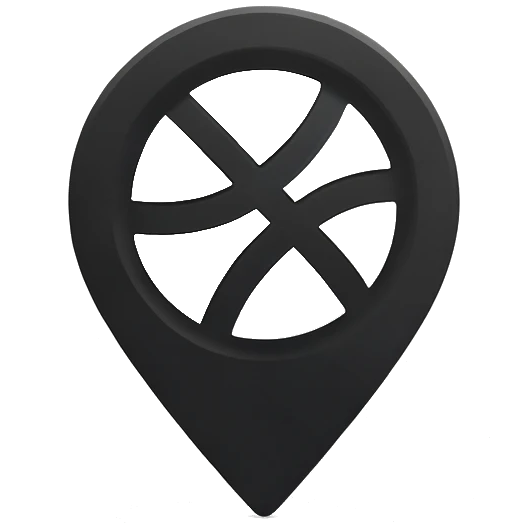
\includegraphics[width=0.3\textwidth]{img/logo.png}
         
        \vspace{3cm}
        \textbf{\Large Giovanni Spadaccini}\\
        \vspace{0.5cm}
        giovanni.spadaccini3@studio.unibo.it
        
        \vfill

    \end{center}
\end{titlepage}

\tableofcontents
\newpage

\section{Introduzione}

Sport Mate è un'applicazione progettata per organizzare e partecipare ad eventi sportivi nella propria zona.

L'obiettivo principale è quello di facilitare la connessione tra appassionati di sport, permettendo loro di creare, trovare e partecipare a varie attività sportive.

\section{Scelta delle tecnologie}

Dart è un buon linguaggio per diverse ragioni. È stato progettato per essere semplice e produttivo, con una sintassi chiara e coerente che facilita la scrittura e la manutenzione del codice.
Inoltre, Dart offre prestazioni elevate grazie alla sua compilazione ahead-of-time (AOT) che consente di produrre codice nativo efficiente.

Flutter è preferibile a React Native per alcuni motivi chiave. Prima di tutto, Flutter offre una maggiore coerenza e controllo sull'aspetto e il comportamento delle applicazioni, grazie al suo set completo di widget personalizzabili.
Inoltre, Flutter utilizza il motore grafico Skia, che garantisce prestazioni elevate e un rendering fluido su tutte le piattaforme. 
Infine, Flutter ha un supporto eccellente per lo sviluppo multi-piattaforma, permettendo di scrivere una sola volta il codice e distribuirlo su iOS, Android, web e desktop.


Per quanto riguarda il backend è stato scritto in python con fastApi, e un database postgrest.

\newpage
\section{Features dell'applicazione}

L'applicazione comprende diverse pagine chiave:

\begin{itemize}
    \item \textbf{Login}: Pagina di accesso per autenticare gli utenti.
    \item \textbf{Signup}: Pagina di accesso creare un profilo utente.
    \item \textbf{Search}: Motore di ricerca per trovare eventi o partner sportivi nella tua zona, con possibilità d'impostare dei filtri. Supporta due modalità di visualizzazione:
    \begin{itemize}
        \item \textbf{Mappa}: visualizza gli eventi con attraverso la loro posizione nella geografica
        \item \textbf{Lista}: lista che permette di visualizzare con più dettagli gli eventi nella zona selezionata
    \end{itemize}
    \item \textbf{Creazione Attività}: Interfaccia per creare nuovi eventi sportivi.
    \item \textbf{Storico}: Raccolta degli eventi passati a cui si è partecipato con la possibilità di aggiungere un feedback o anche chiamato ricordo.
    \item \textbf{Ricordo}: Sezione per lasciare un messaggio di ricordo dell'attività, e aggiungerci un punteggio su quanto è stata gradita.
    \item \textbf{Visualizzazione di un'Attività e Partecipazione}: Pagina dettagliata di ogni evento, che include opzioni per iscriversi all'evento, ottenere informazioni aggiuntive e aggiungere una notifica per ricordarsi dell'evento.
\end{itemize}

\newpage
\section{Struttura del codice sorgente}


\begin{wrapfigure}{r}{0.40\textwidth}
    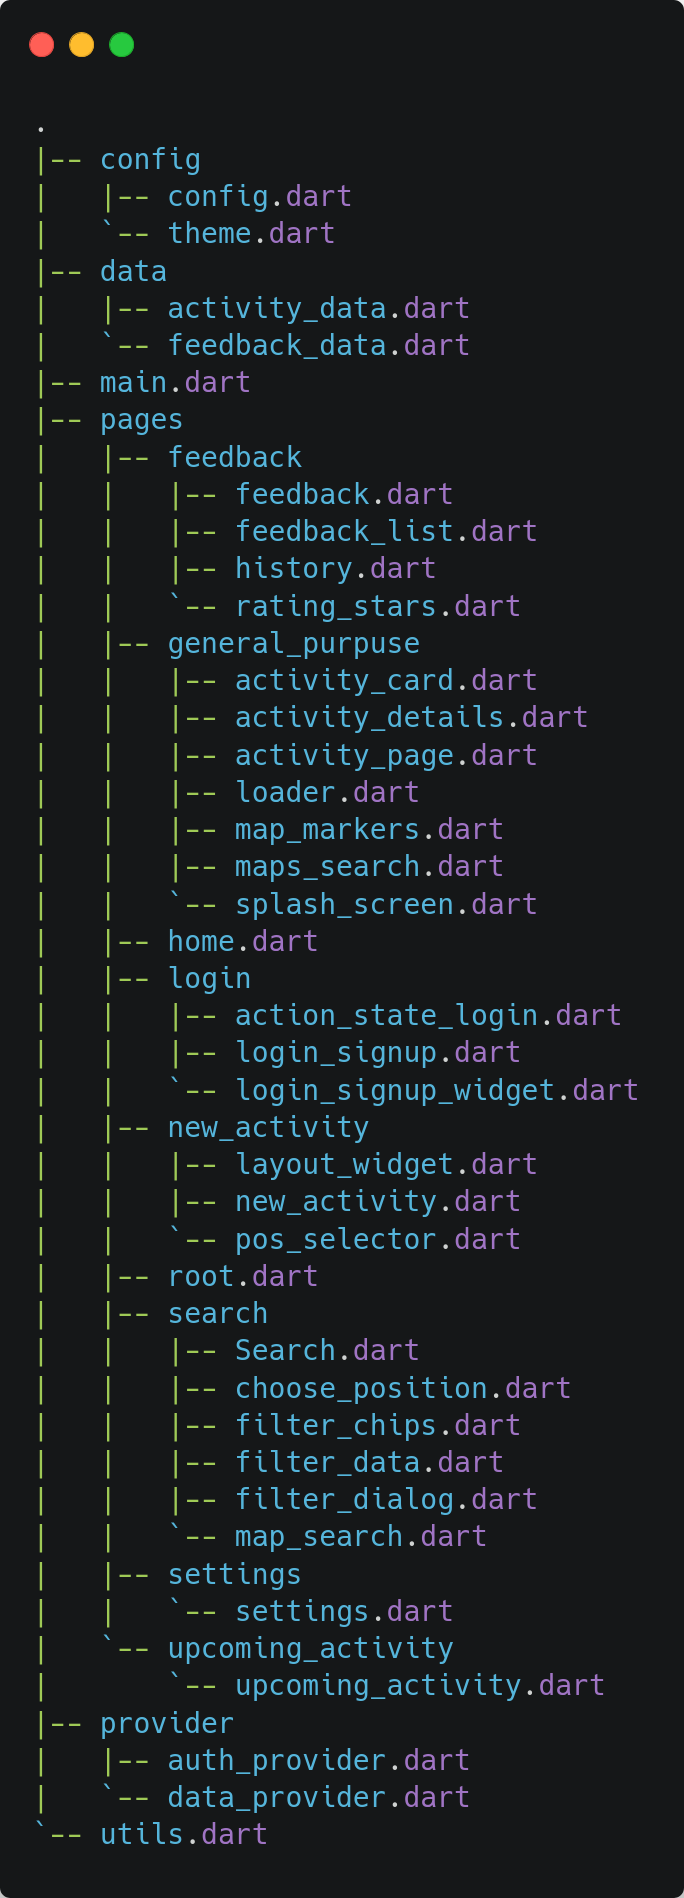
\includegraphics[width=0.35\textwidth]{img/tree_structure.png}
    \vspace{-45pt}
\end{wrapfigure}
La struttura del codice sorgente è divisa nelle seguenti cartelle:\\

\begin{itemize}
\item \textbf{config}: Contiene le configurazioni globali dell'applicazione che non cambiano durante l'esecuzione, o che se cambiano non hanno un'influenza sulla UI
    \item \textbf{data}: Contiene le strutture dati delle activity e del feedback.
    \item \textbf{provider}: Contiene i dati che, quando cambiano, hanno un riscontro nella UI e quindi dev'essere aggiornata anche la UI. 
    \item \textbf{pages}: Sono definiti tutti i widget delle varie pagine e le pagine stesse. 
    \item \textbf{utils.dart}: Contiene utility functions utilizzate in varie parti dell'applicazione.
\end{itemize}


I dati vengono caricati da un backend facendo richieste progressive (che si aggiornano rispetto all'ultima richiesta fatta) e vengono salvati in locale, così da averli offline.


\newpage
\section{Scelte implementative}

\subsection{Dati}

Le due strutture di dati principali dell'applicazione sono definite sotto \textbf{data} e sono:

% create two image row
\begin{figure}[h]
    \centering
    \begin{minipage}{0.45\textwidth}
        \centering
        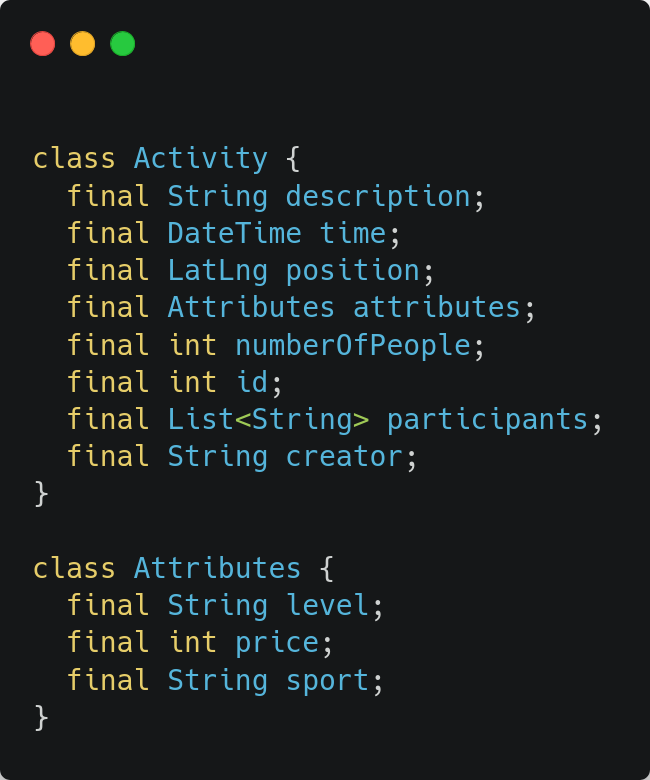
\includegraphics[width=0.9\linewidth]{img/activity.png}
    \end{minipage}\hfill
    \begin{minipage}{0.45\textwidth}
        \centering
        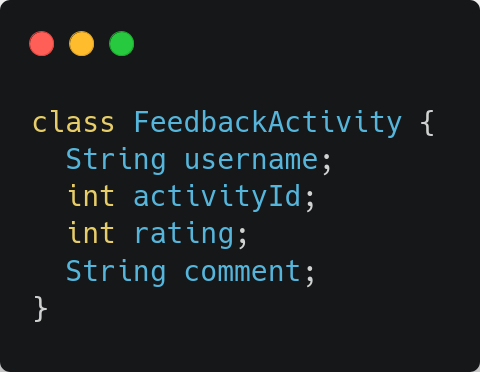
\includegraphics[width=0.9\linewidth]{img/feedback.png}
    \end{minipage}
\end{figure}


\begin{itemize}
    \item \textbf{Activity}~\ref{gl:activity}: contiene i dati relativi ad un evento sportivo, come il nome, la descrizione, la posizione, la data e l'ora, il numero di partecipanti, ecc.
    \item \textbf{Feedback}~\ref{gl:feedback}': contiene i dati relativi al feedback lasciato da un utente su un'attività, come il punteggio, il messaggio e l'attività  associata. 
\end{itemize}

\newpage

\subsection{Provider}

\begin{wrapfigure}{r}{0.64\textwidth}
    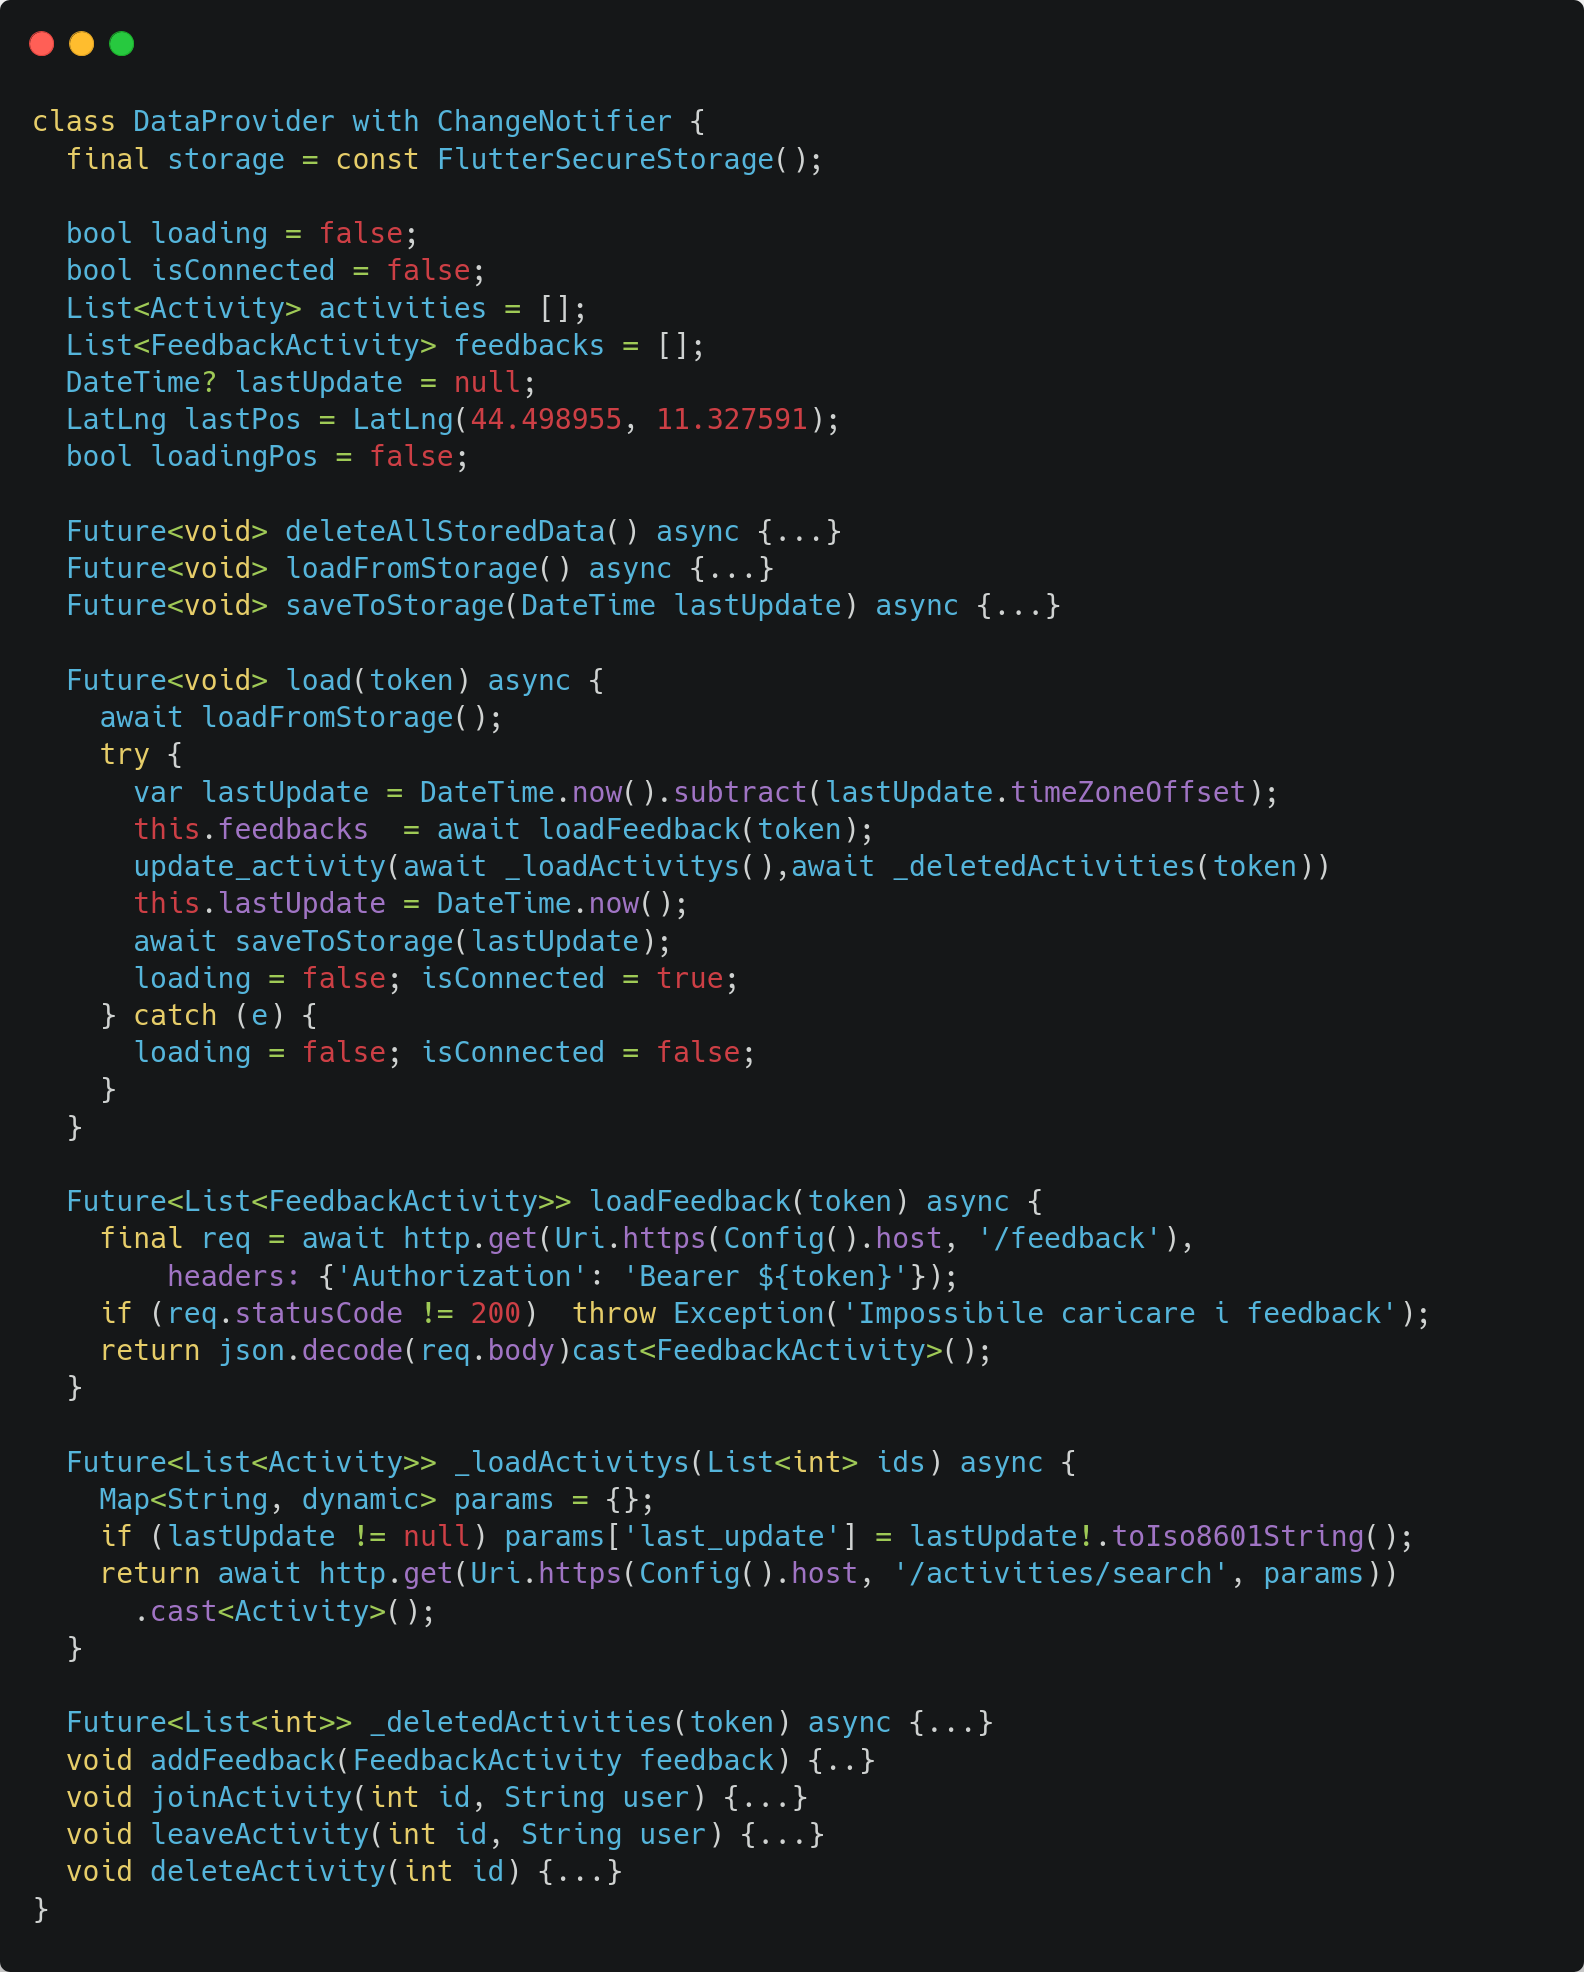
\includegraphics[width=0.63\textwidth]{img/data_provider.png}
\end{wrapfigure}
Un provider in Flutter è una classe che gestisce e fornisce dati e stato all'applicazione, facilitando la separazione tra logica di business e interfaccia utente. Questo approccio migliora la leggibilità e la manutenzione del codice. Il provider viene inserito nel widget tree e consente a ogni widget di accedere e reagire agli aggiornamenti dello stato. Utilizzando il provider, si può garantire una gestione efficiente e reattiva dei dati, poiché i widget si aggiornano automaticamente quando il provider notifica un cambiamento di stato. 

Nell'applicazione, come visto nella sezione di struttura del codice sorgente, ne abbiamo due:

\begin{itemize}
    \item \textbf{Activity Data}: specifica i metodi e i dati per caricare, modificare ed eliminare i dati relativi alle Activity~\ref{gl:activity}
    \item \textbf{Auth}: specifica i metodi e i dati per gestire l'autenticazione e l'accesso dell'utente.
\end{itemize}

\textbf{Activity Data} in particolare è un provider che si occupa di caricare i dati delle activity, e di salvarli in locale, così da averli offline.
Implementa la politica Single Source of Truth, ovvero che i dati vengono caricati da un backend facendo richieste progressive (che si aggiornano rispetto all'ultima richiesta fatta) e vengono salvati in locale, così da averli offline.

\textbf{Auth} questo provider permette di aggiornare tutta la UI quando l'utente si autentica o si disconnette.

\newpage

\subsection{Pagine}

\subsubsection{Home}


All'esecuzione carica il file home, che controlla se è stato salvato un authetication token valido, se sì carica la pagina Search~\ref{sec:search}, se no carica la pagina di Registrazione e Login~\ref{sec:login}. Il cambio è fatto attraverso provider che, in base al cambiamento del token sceglie quale pagine caricare.

Quindi il codice della homepage è qualcosa come:

\begin{figure}[h]
    \centering
        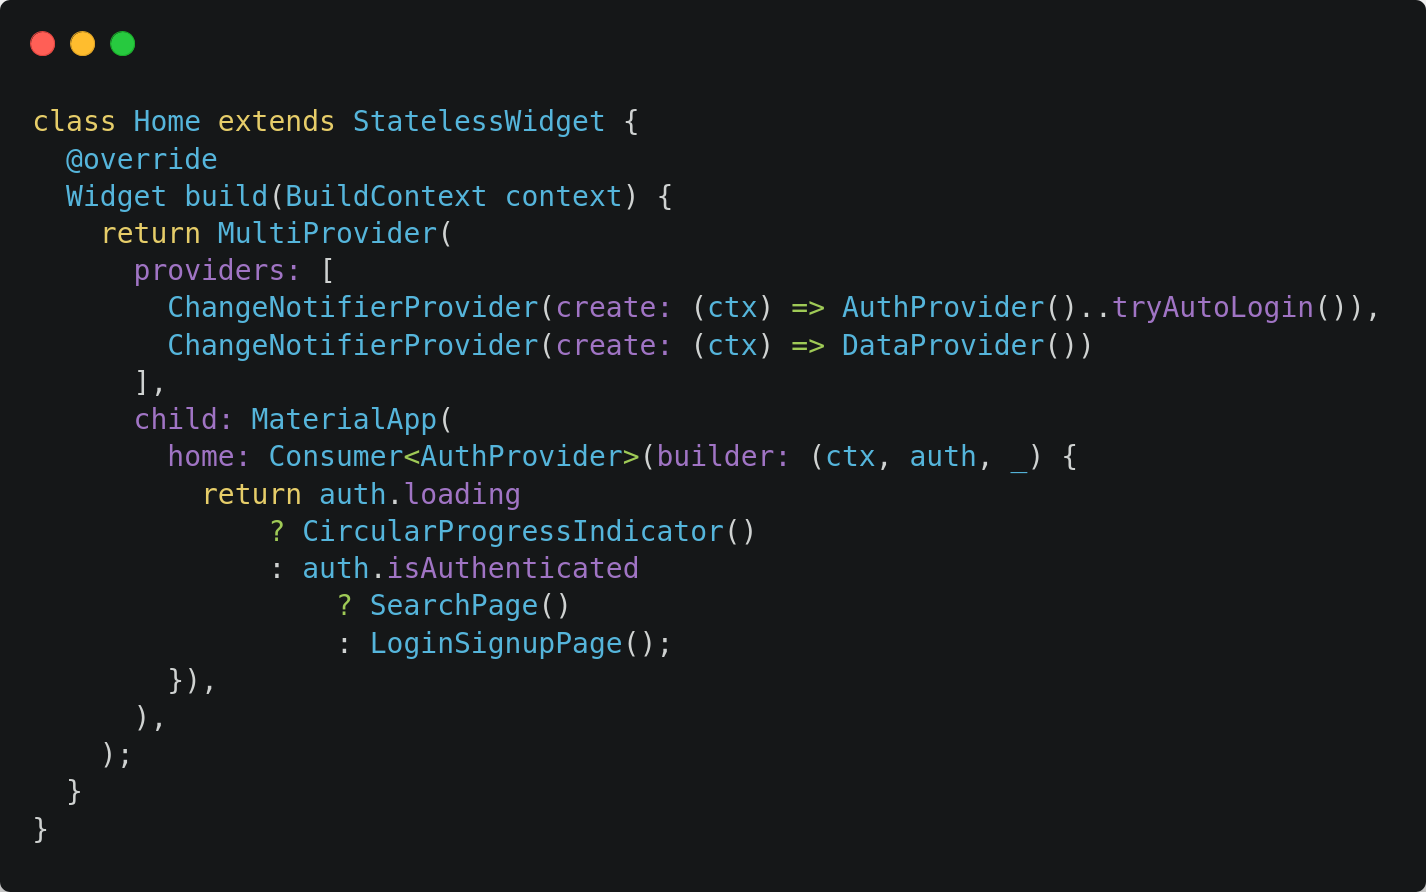
\includegraphics[width=0.9\linewidth]{img/home.png}
\end{figure}


Inoltre nella home andiamo a definire anche il DataProvider che utilizzeremo dopo.

\newpage

\subsection{Registrazione e Accesso}
\label{sec:login}

Le prime pagine che si incontrano sono quelle di accesso e registrazione, queste pagine si connettono alle api e impostano l'authetication token attraverso l'auth provider, questo fa aggiornare la home page cambiando la pagina home a SearchPage~\ref{sec:search}.

\begin{figure}[H]
    \begin{minipage}{0.40\textwidth}
        \centering
        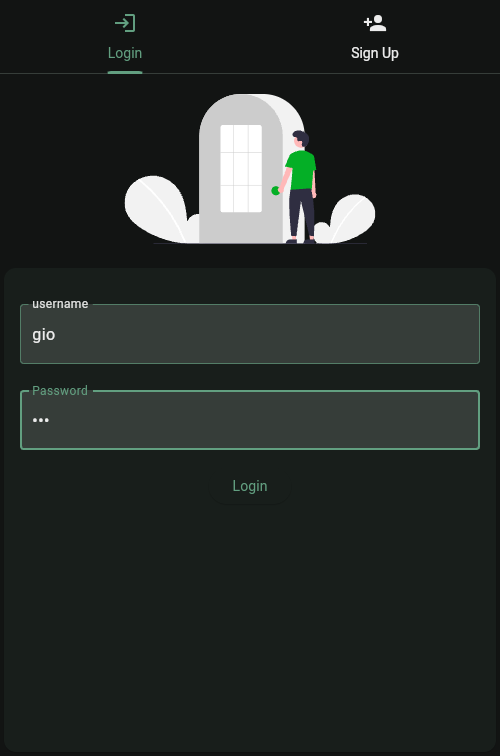
\includegraphics[width=0.8\linewidth]{img/login.png}
    \end{minipage}\hfill
    \begin{minipage}{0.40\textwidth}
        \centering
        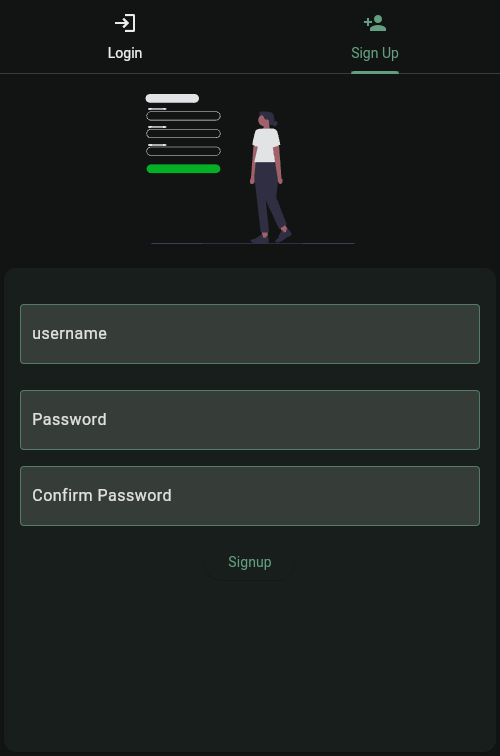
\includegraphics[width=0.8\linewidth]{img/registrazione.png}
    \end{minipage}
\end{figure}



\subsection{Search}
\label{sec:search}

Search è la pagina più complessa dell'applicazione, permette di cercare eventi sportivi nella propria zona, con possibilità d'impostare dei filtri. Supporta due modalità di visualizzazione: Vediamo il codice ad alto livello, è composto da due widget stateful, il primo \textbf{SearchPage} che è un wrapper, carica i dati da DataProvider e aggiorna \textbf{\_SearchPage} che contiene l'interfaccia della search.
\textbf{SearchPage} è il widget root della pagine autenticate, questo significa che quando si modificano dei dati significativi in Data Provider, questo aggiorna tutti i componenti sottostanti.

La \textbf{\_SearchPage} contiene altri dati come i filtri, la posizione attuale, e il raggio di ricerca.
% todo specifica che è la pagina root quando uno è autenticato quindi i dati di DataProvider sono condivisi con tutte le altre pagine 

\begin{figure}[H]
    \begin{minipage}{0.49\textwidth}
        \centering
        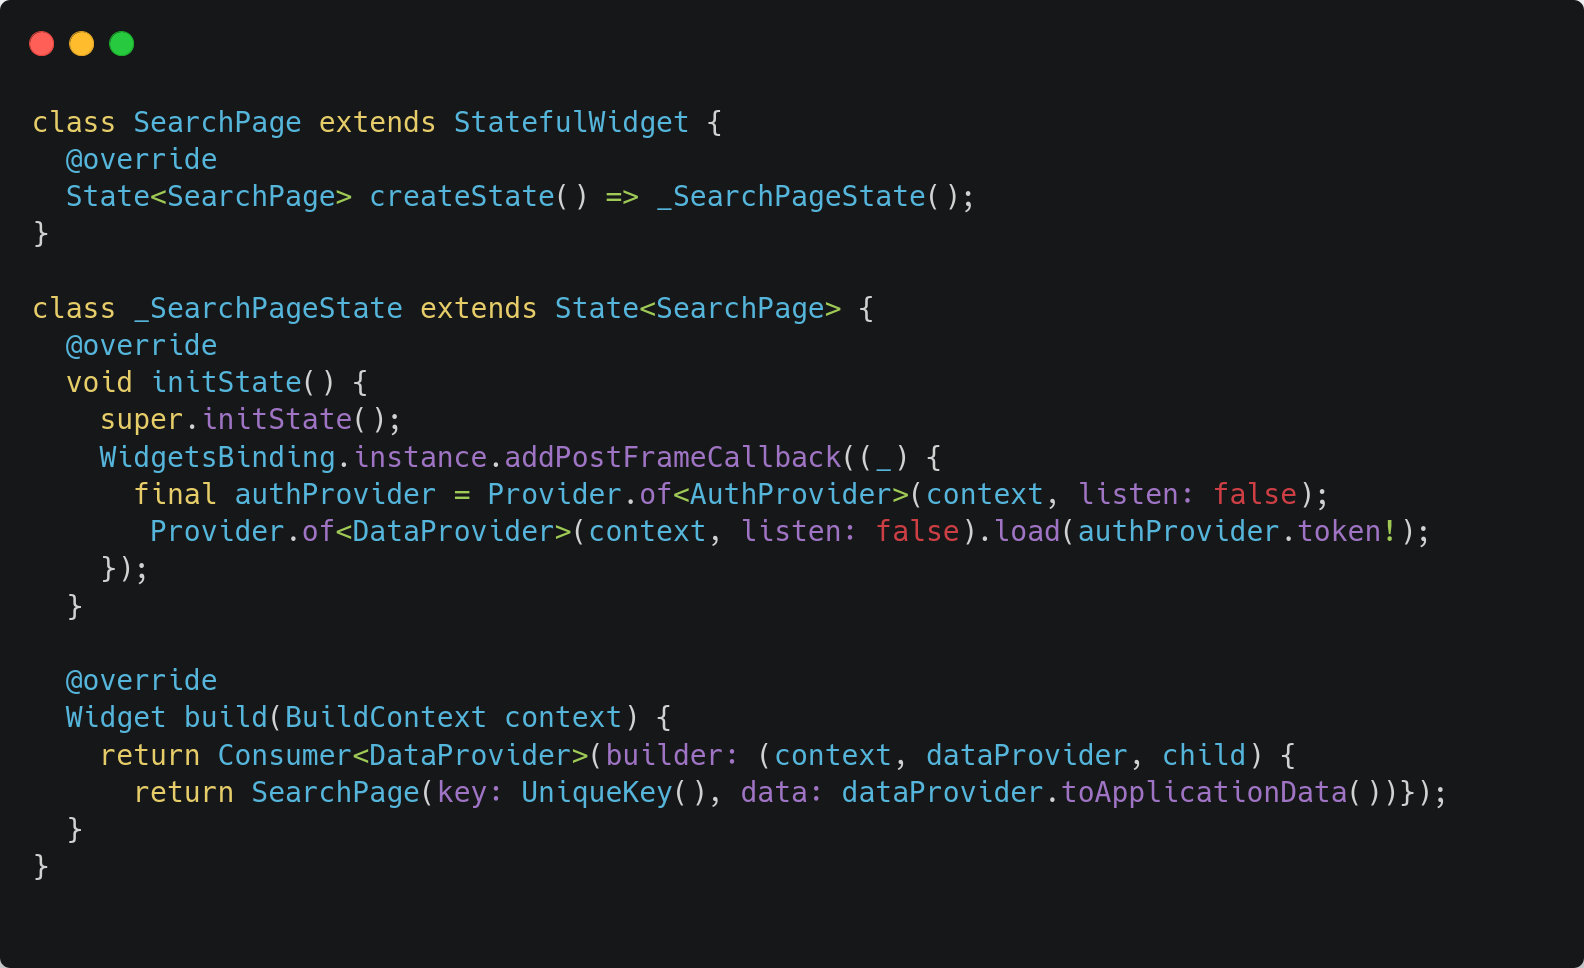
\includegraphics[width=1\linewidth]{img/search_page.png}
    \end{minipage}\hfill
    \begin{minipage}{0.49\textwidth}
        \centering
        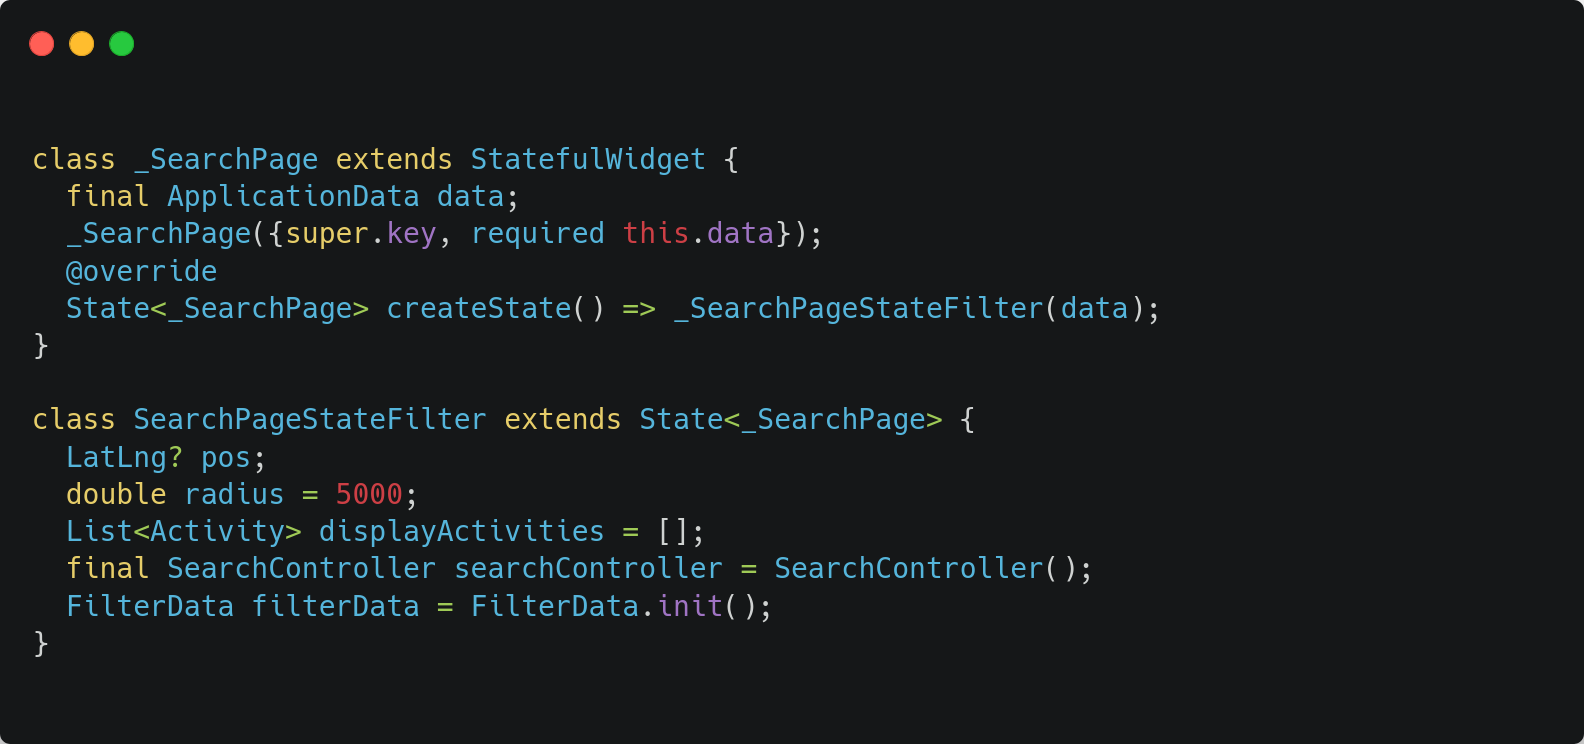
\includegraphics[width=1\linewidth]{img/search_state.png}
    \end{minipage}
\end{figure}

In search possiamo compiere varie azioni, tra cui visualizzare le attività sia in modalità lista~\ref{fig:search_list}, che in modalità mappa~\ref{fig:search_map}, permette di visualizzare gli eventi sia tramite la posizione.
Infatti nella modalità mappa posiamo visualizzare gli eventi cliccando sul marker.
I filtri agiscono invece su entrambe le visualizzazioni degli eventi.

\begin{figure}[h]
    \begin{minipage}{0.32\textwidth}
        \centering
        \label{fig:search:map}
        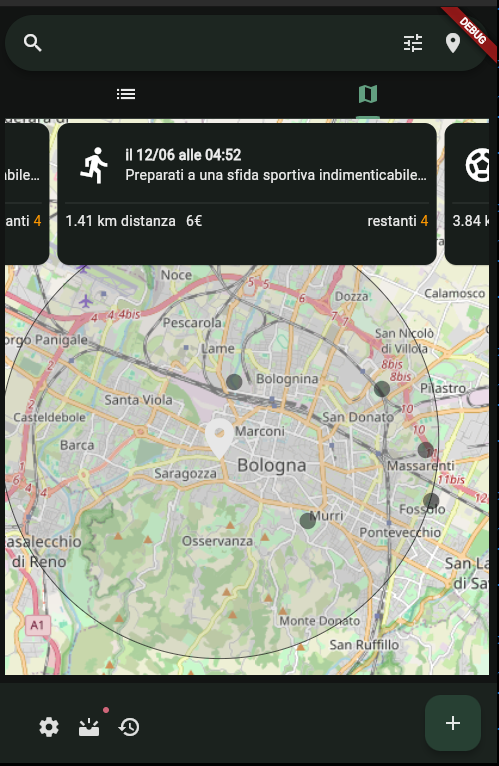
\includegraphics[width=1\linewidth]{img/search_map_page.png}
    \end{minipage}
    \begin{minipage}{0.32\textwidth}
        \centering
        \label{fig:filter}
        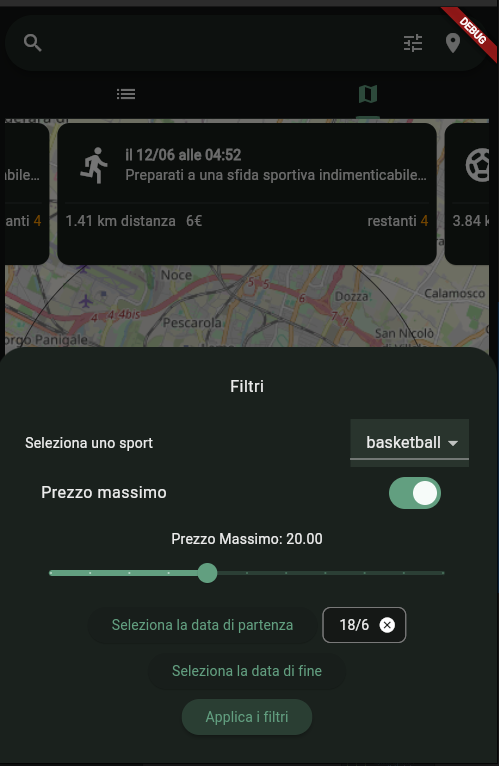
\includegraphics[width=1\linewidth]{img/filter.png}
    \end{minipage}
    \begin{minipage}{0.32\textwidth}
        \label{fig:search_list}
        \centering
        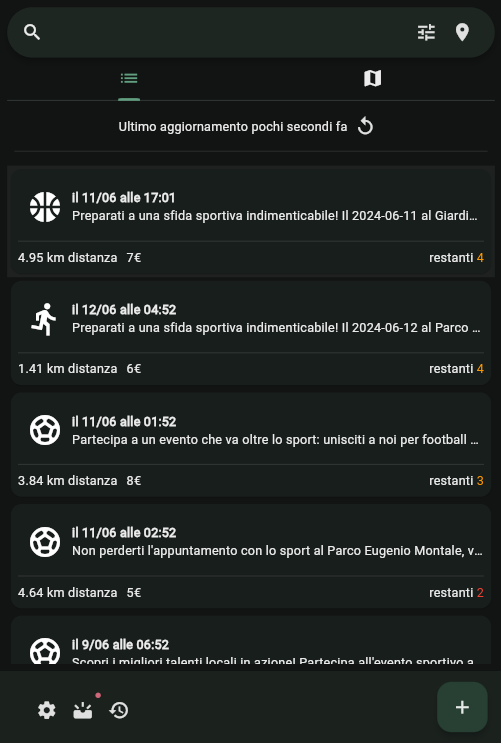
\includegraphics[width=1\linewidth]{img/Search.png}
    \end{minipage}
\end{figure}

Di default la posizione e raggio sono preimpostati a Bologna o all'ultima posizione da cui è avvenuto l'ultimo accesso.
Per cambiarla si può cliccare sul bottone in alto a destra con il simbolo dell'puntatore, questo porta ad un altra pagina che permette di cambiare la posizione e il raggio di ricerca.
E trascinando la mappa si può cambiare la posizione e il raggio di ricerca tramite lo slider.
Inoltre si può anche cercare una posizione tramite la barra di ricerca, o impostare quella corrente con il simbolo della posizione accanto.

Oltre i filtri si può usare anche la barra di ricerca per cercare un'attività tramite la descrizione.

\begin{figure}[h]
    \begin{minipage}{0.32\textwidth}
        \centering
        \label{fig:search_map}
        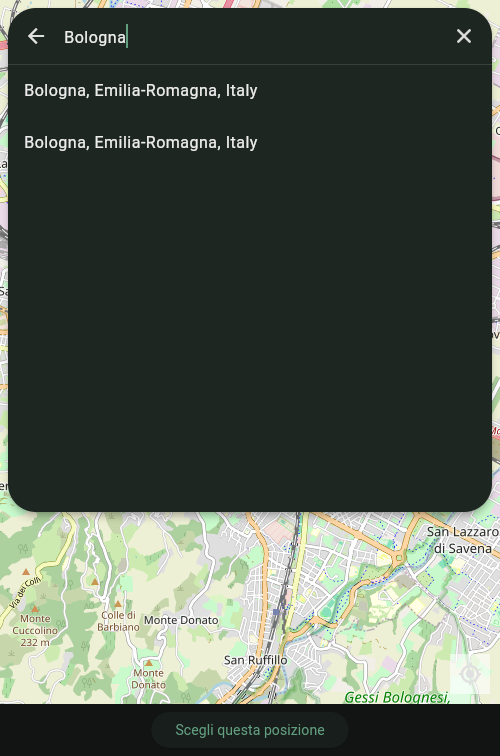
\includegraphics[width=1\linewidth]{img/search_map.png}
    \end{minipage}
    \begin{minipage}{0.32\textwidth}
        \centering
        \label{fig:select_radius}
        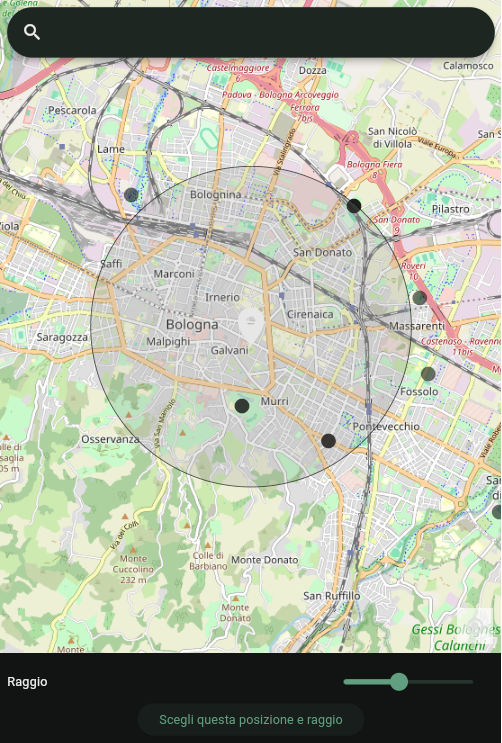
\includegraphics[width=1\linewidth]{img/select_radius.png}
    \end{minipage}
    \begin{minipage}{0.32\textwidth}
        \centering
        \label{fig:select_radius}
        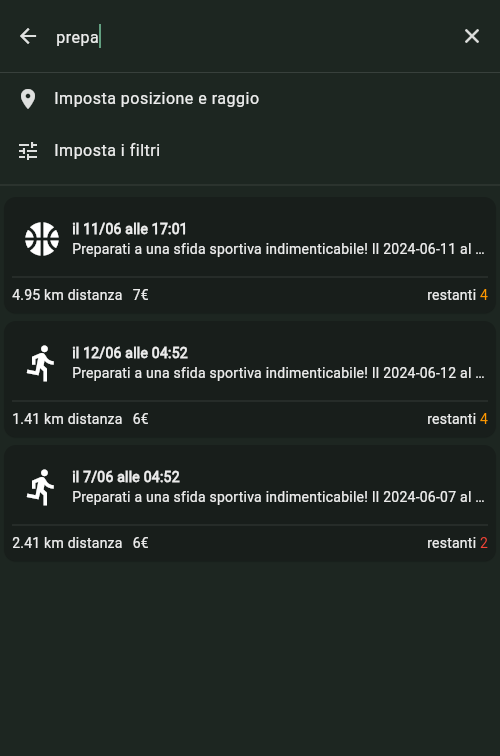
\includegraphics[width=1\linewidth]{img/search_activity.png}
    \end{minipage}
\end{figure}

\subsection{Aggiungi attività}

La creazione nel creare un attività sportiva sono diverse pagine da completare per creare un evento sportivo:
\begin{itemize}
    \item \textbf{Posizione}: permette di selezionare la posizione dell'evento attraverso una mappa.
    \item \textbf{Data}: permette di selezionare la data e l'ora dell'evento.
    \item \textbf{Dettagli}: permette di inserire una descrizione dell'evento, lo sport, il numero di partecipanti e il prezzo.
\end{itemize}


\begin{figure}[H]
    \begin{minipage}{0.32\textwidth}
        \centering
        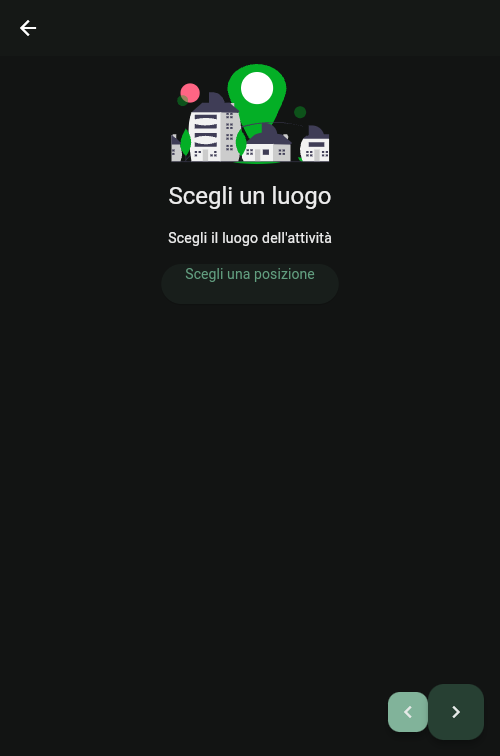
\includegraphics[width=1\linewidth]{img/new_pos.png}
    \end{minipage}
    \begin{minipage}{0.32\textwidth}
        \centering
        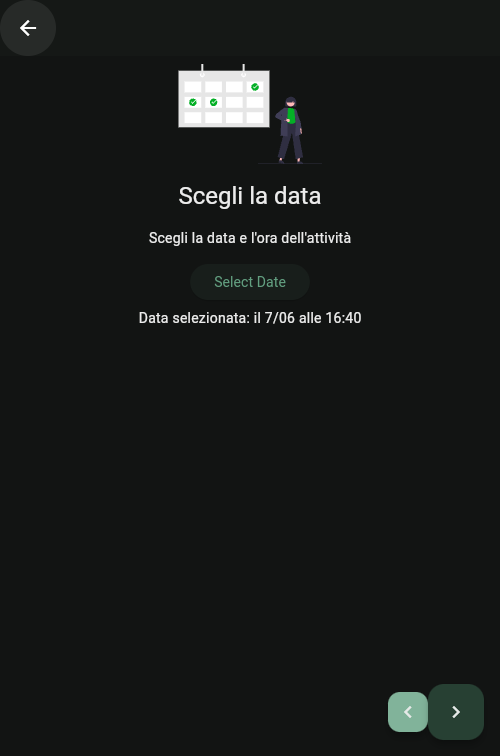
\includegraphics[width=1\linewidth]{img/new_date.png}
    \end{minipage}
    \begin{minipage}{0.32\textwidth}
        \centering
        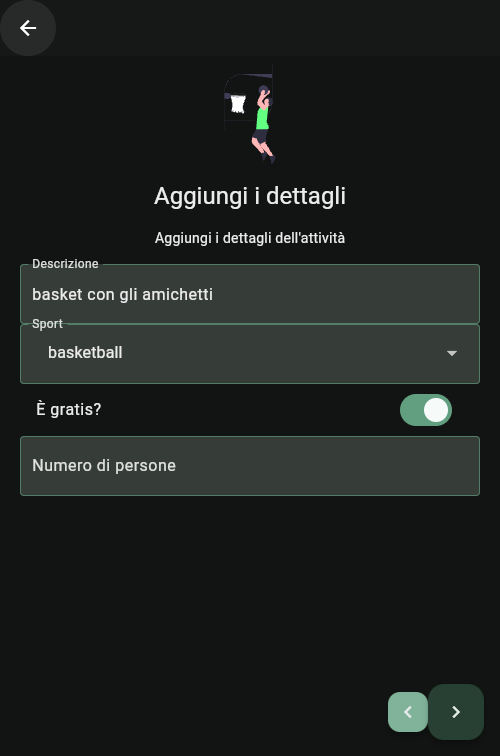
\includegraphics[width=1\linewidth]{img/new_desc.png}
    \end{minipage}
\end{figure}

\subsection{Partecipa ad un'attività}

Per partecipare ad un'attività basta cliccare sul bottone partecipa, e si verrà aggiunti alla lista dei partecipanti. Inoltre si può aggiungere un promemoria per l'evento.
Questo promemoria verrà aggiunto tramite notifica che verrà inviata \textsf{n} minuti prima dell'evento, dove \textsf{n} sono i minuti definiti nelle impostazioni.


\begin{figure}[H]
    \centering
    \begin{minipage}{0.32\textwidth}
        \centering
        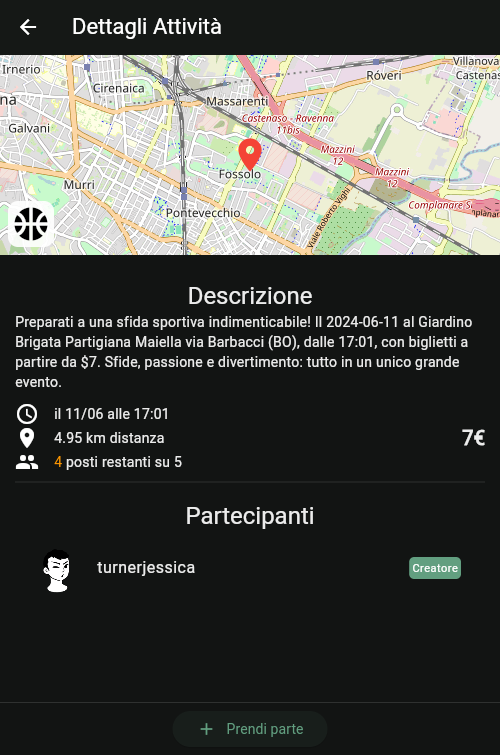
\includegraphics[width=1\linewidth]{img/descrizione.png}
    \end{minipage}
    \begin{minipage}{0.32\textwidth}
        \centering
        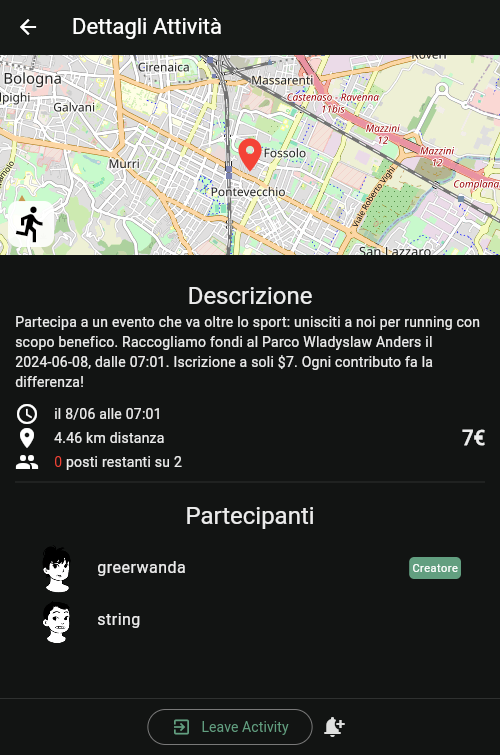
\includegraphics[width=1\linewidth]{img/joined.png}
    \end{minipage}
\end{figure}

\subsection{Storia}

Permette di visualizzare gli eventi passati a cui si è partecipato con il relativo Ricordo, o di aggiungerlo in caso non lo si abbia fatto. 
Quando aggiunge un feedback utilizza il provider per aggiornare i dati sia in locale che nel backend.


\begin{figure}[H]
    \centering
    \begin{minipage}{0.32\textwidth}
        \centering
        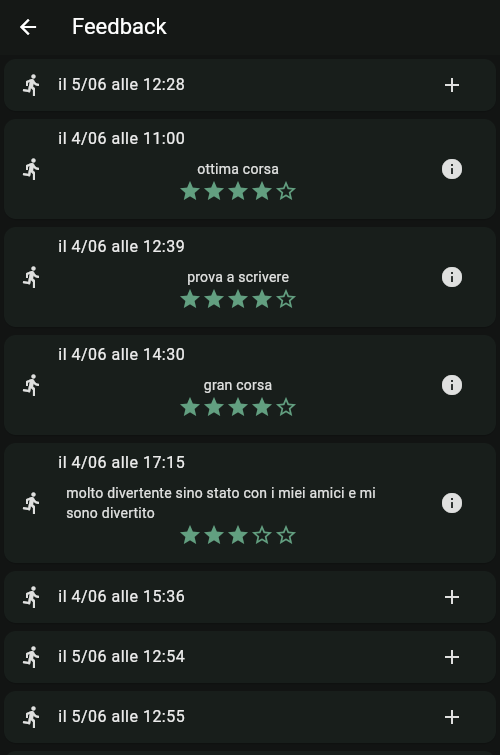
\includegraphics[width=1\linewidth]{img/history.png}
    \end{minipage}
    \begin{minipage}{0.32\textwidth}
        \centering
        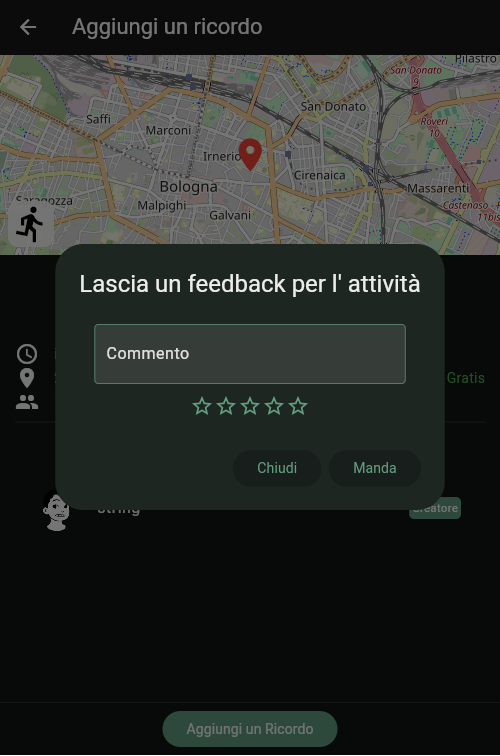
\includegraphics[width=1\linewidth]{img/add_feedback.png}
    \end{minipage}
\end{figure}


\subsection{Impostazioni}

\begin{wrapfigure}{r}{0.50\textwidth}
    \vspace{-26pt}
    \center
    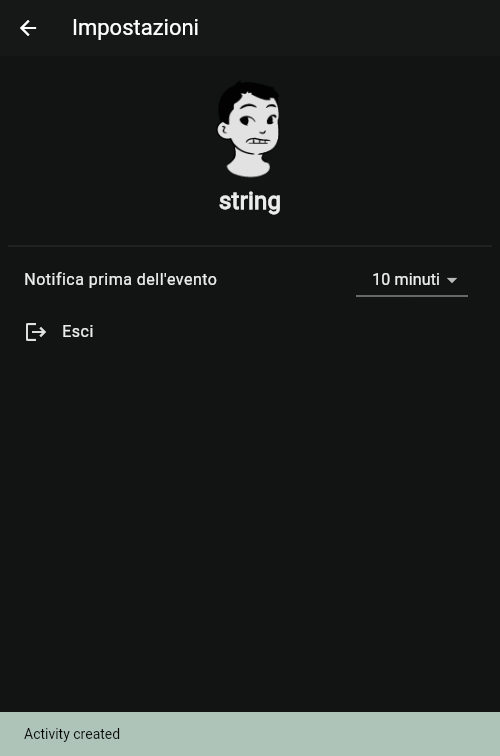
\includegraphics[width=0.5\linewidth]{img/settings.png}
\end{wrapfigure}
Le impostazioni, mostrano informazioni sull'utente, e permettono di modificare le impostazioni che per ora è solo quanto prima dell'evento ricevere una notifica. Inoltre permette di disconnettersi.
Le configurazioni a differenza di altre impostazioni non devono essere inserite dentro un Provider in quanto non influenzano la UI.





\end{document}
